\section{Einleitung}

\subsection{Vorstellung des Unternehmens}
Die Arbeit wurde in Zusammenarbeit mit der \koorperationsunternehmen~angefertigt. Dieses Unternehmen verwaltet die informationstechnischen und finanziellen Aufgaben der Polipol Gruppe. Die Polipol Gruppe wurde 1990 gegründet und produziert heute als einer der führenden Polstermöbelhersteller Europas für den weltweiten Markt. Zum Sortiment gehören Sofas, Sessel und Polsterbetten. Die Produktionsstandorte liegen in Polen, Rumänien, Belarus und Deutschland. Die Kunden der Polipol Gruppe sind in erster Linie Möbelhäuser. Diese vertreiben die Garnituren dann weiter an die Endkunden.

\subsection{Ausgangssituation und Motivation}
% Quellen:
% Möbelumsatz (Nur zur Info) - https://de.statista.com/statistik/daten/studie/260915/umfrage/marktvolumen-fuer-moebel-in-deutschland/
% eCommerce im Möbelhandel (auch wenn wachsend, sehr gering) - https://de.statista.com/statistik/daten/studie/260586/umfrage/umsatzanteil-des-ecommerce-im-moebelhandel-in-deutschland/
% Einkaufsverhalten Generationen beim Möbelkauf - https://de.statista.com/statistik/daten/studie/866795/umfrage/kaufverhalten-beim-moebelkauf-nach-generationen-in-deutschland/

Wie in Abbildung \ref{fig:furniture_market_ecommerce} zu sehen ist, machte der Online-Möbelhandel bis 2018 nur {3,3\%} vom Umsatz des Möbeleinzelhandels aus. Gerade ältere Menschen geben an, zum Großteil Möbel im stationären Einzelhandel zu kaufen. Aber auch die Generation der \enquote{Millenials} und die \enquote{Generation Z} kaufen Möbel noch überwiegend direkt vor Ort.\footnote{\cite[Vgl.][]{Statista2021b}} Der meistgenutzte Verkaufspunkt ist damit der Einzelhandel. Und gerade dort ist eine kompetente und persönliche Beratung durch Verkäufer die wichtigste Informationsquelle. Informationen zu den verfügbaren Modellen, Bezügen (Stoff und Leder) und deren Eigenschaften sowie mögliche Kombinationen mit Funktionen (z. B. Armteilverstellung, Bettfunktion, Höhenverstellbar etc.) erhalten die Verkäufer von den Herstellern. Mit einer App soll der Verkäufer Zugriff auf diese Informationen in einem mobilen Format bekommen. So kann auch flexibel direkt am Sofa und nicht nur vom Computer aus beraten werden. Es fehlt den Verkäufern aktuell an einer mobilen Wissensdatenbank.

\begin{figure}[hbt]
    \centering
    \begin{minipage}[t]{.9\textwidth}
        \caption{Umsatzanteil des eCommerce im Einzelhandel mit Wohnmöbeln in Deutschland in den Jahren 2005 bis 2018}
        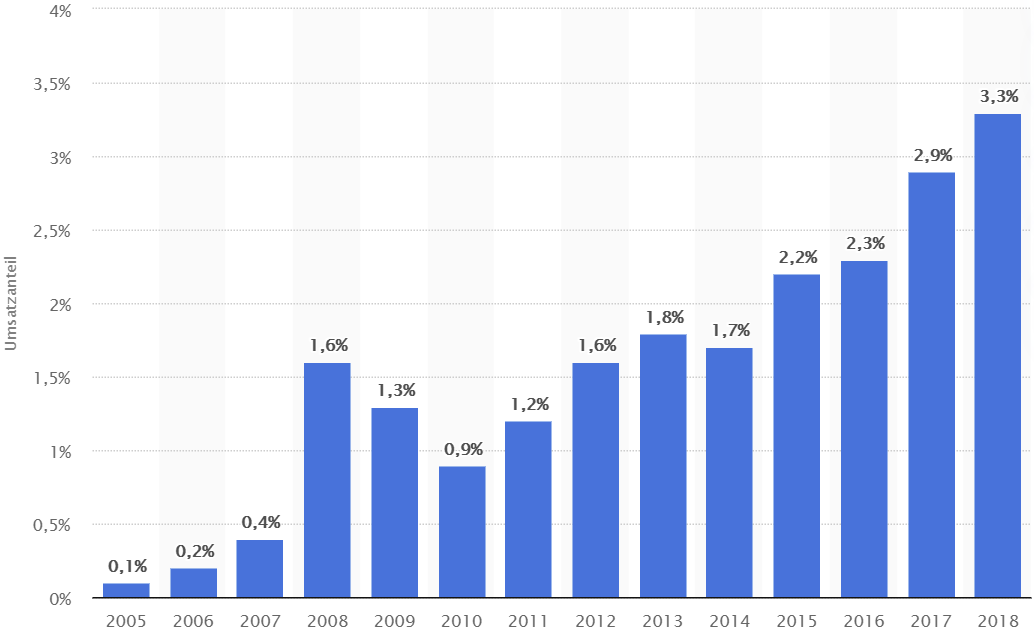
\includegraphics[width=1\textwidth]{img/Umsatzanteil_eCommerce_Moebeleinzelhandel.PNG}\\
        \source{\cite{Statista2021a}}
        \label{fig:furniture_market_ecommerce}
    \end{minipage}
\end{figure}

\subsection{Ziel}
Ziel dieser Arbeit ist die Entwicklung eines Prototypen in Form einer Android-App. Dieser soll später als Vorlage für die Entwicklung einer App dienen. Mit dem Prototypen soll Feedback zu den enthaltenen Funktionen und deren Umsetzung gesammelt werden. Außerdem soll bei der Entwicklung bereits viel Wert auf das Design und die Benutzererfahrung gelegt werden, um sich möglichst früh auf eine Benutzeroberfläche zu einigen. Zielgruppe der App sind später die Verkäufer in den Möbelhäusern. Mit der App sollen sie in ihrem Alltag unterstützt werden und die Endkunden effektiver beraten können. Es soll zudem eine stärkere Bindung zwischen der Polipol-Gruppe und den Verkäufern aufgebaut werden. Zur Beratung sollen die Verkäufer detaillierte Informationen über Garnituren, Bezüge und verfügbare Modellfunktionen in der App erhalten. Zur Veranschaulichung sollen auch visuelle Elemente wie Bilder und Videos eingebaut werden. Die App soll eine mobile Wissensdatenbank zur Beratung der Endkunden darstellen.

\subsection{Aufbau und Struktur}
In dieser Arbeit werden zuerst die Grundlagen erläutert. Dazu zählen die Themen Smartphone, Apps und das Betriebssystem Android. Dann wird in  der Konzeption auf die Anforderungsanalyse in Form von User-Stories und die Planung der Entwicklung eingegangen. In der Umsetzung wird sich dann an den User-Stories orientiert. Dabei werden die zentralen Seiten beschrieben und Besonderheiten in der Implementierung erläutert. In Kapitel \ref{sec:feedback} wird dann auf das gesammelte Feedback eingegangen. Zum Schluss wird mit einer kurzen Zusammenfassung ein Fazit gebildet und ein Ausblick über die Einarbeitung des Feedbacks und mögliche Weiterentwicklungen gegeben.

\clearpage